\section{Homework Solutions (Yip)}
These are the solutions to Yip's Math/Stat 519 homework for the fall
semester of 2016.

Our main reference is \cite{ross}.

\subsection{Homework 1}
\subsubsection{Problems}
\begin{problem}[Ross, \S 1, \# 7]
  \hfill
  \begin{alphlist}
  \item In how many different ways can \(3\) boys and \(3\) girls sit in a
    row?
  \item In how many ways can \(3\) boys and \(3\) girls sit in a row if the
    boys and the girls are each to sit together?
  \item In how many ways if only the boys must sit together?
  \item In how many ways if no two people of the same sex are allowed to
    sit together?
  \end{alphlist}
\end{problem}
\begin{solution*}
  For the problems that follow, we will not justify our answer but instead
  we make a note here that they are consequences of the general principle
  of counting introduced in the book.
  \\\\
  For part (a), there are \(6!\) ways of arranging \(3\) boys and \(3\)
  girls (\(6\) children).
  \\\\
  For part (b), assuming the author meant ``there is at least one girl next
  to every boy'' by ``the boys and girls must sit together'' we have
  \(2(3!)^2\) ways to arrange the \(3\) boys and \(3\) girls in this way
  (the \(2\) comes from the choice of placing a boy or a girl first).
  \\\\
  For part (c), assuming the author means that ``it does not matter in
  which order the boys sit, but they must sit together'' we have \(4(3!)\)
  where the \(3!\) comes from the different ways we can arrange the \(3\)
  girls and the \(4\) from the different ways we can place \(3\) boys
  contiguously on a row with \(6\) slots.
  \\\\
  For part (d), we can either start with a boy or a girl, which gives us a
  factor of \(2\), and once that choice has been made, the rest of the
  spots are reserved for boys/girls alternating from one to the other to
  the end of the row; that is, they are completely determined except for
  the particular boy or girl that is to take those spots. Next for each
  spot, we have \(3\) choices of boy (respectively, girl) which gives us a
  \(3!\) factor. Thus, the number of ways in which we can do this is
  precisely \(2(3!)^2\).
\end{solution*}

\begin{problem}[Ross, \S 1, \# 11]
  In how many ways can \(3\) novels, \(2\) mathematics books, and \(1\)
  chemistry book be arranged on a bookshelf if
  \begin{alphlist}
  \item the books can be arranged in any order?
  \item the mathematics books must be together and the novels must be
    together?
  \item the novels must be together, but the other books can be arranged in
    any order?
  \end{alphlist}
\end{problem}
\begin{solution*}
  For part (a), if the \(3+2+1=6\) books can be arranged in any order,
  there are \(6!\) arrangements.
  \\\\
  For part (b), let us first count the different ways we can arrange \(3\)
  blocks of books. There are \(3!\) different ways to arrange these and
  once this arrangement has been made, \(3!2!\) ways to arrange the \(3\)
  novels and \(2\) mathematics books. Thus, there are \((3!)^22!\) ways of
  arranging the \(6\) books subject to these restrictions.
  \\\\
  For part (c), if the novels must be together, we must first count the
  different number of ways we can put a contiguous row of \(3\) books in
  \(6\) slots. The answer to that problem is \(4\). Now, assuming the
  arrangement of the \(3\) novels does not matter, we have \(4\cdot 3!\)
  ways of arranging the rest of the books. If we care about randomizing the
  \(3\) novels themselves, then we have \(4(3!)^2\) distinct arrangements.
\end{solution*}

\begin{problem}[Ross, \S 1, \# 19]
  From a group of \(8\) women and \(6\) men, a committee consisting of
  \(3\) men and \(3\) women is to be formed. How many different committees
  are possible if
  \begin{alphlist}
  \item \(2\) of the men refuse to serve together?
  \item \(2\) of the women refuse to serve together?
  \item \(1\) man and \(1\) woman refuse to serve together?
  \end{alphlist}
\end{problem}
\begin{solution*}
  For part (a), there are
  \[
    \binom{8}{3}\left[\binom{4}{3}+2\binom{4}{2}\right]
  \]
  ways to choose a committee that avoids putting the two men in question
  together. The \(\binom{8}{3}\) comes from the different number of ways we
  can choose \(3\) women from a pool of \(8\) and the
  \(\binom{4}{3}+2\binom{4}{2}\) are the different number of ways we can
  choose \(3\) men to from a pool of \(6\), \(2\) of which refuse to serve
  together; i.e., we can either choose neither of the two men in question,
  giving us \(\binom{4}{3}\) possibilities, or choose one of them giving us
  \(\binom{4}{2}\) possibilities (multiply this by \(2\), this represents
  the choice for one of the \(2\) men).
  \\\\
  For part (b), the exact argument given above yields
  \[
    \binom{6}{3}\left[\binom{6}{3}+2\binom{6}{2}\right]
  \]
  possible committees.
  \\\\
  For part (c), we have \(\binom{5}{3}\binom{7}{3}\) if neither the man nor
  the women in question serve in the committee;
  \(\binom{5}{3}\binom{7}{2}\) if the woman serves; and
  \(\binom{5}{2}\binom{7}{3}\) if the man serves. In total, this is
  \[
    \binom{5}{3}\binom{7}{3}+\binom{5}{3}\binom{7}{2}+\binom{5}{2}\binom{7}{3}.\qedhere
  \]
\end{solution*}

\begin{problem}[Ross, \S 1, \# 21]
  Consider the grid of points show at the top of the next column (in the
  book; we draw it here using Asymptote).
  \[
    
\includegraphics{yip-1-1}
  \]
  Suppose that, starting at the point labeled \(A\), you can go one step up
  or one step to the right at each move. This procedure is continued until
  the point labeled \(B\) is reached. How many different paths from \(A\)
  to \(B\) are possible?

  \noindent\emph{Hint:} Note that to reach \(B\) from \(A\) you must take
  \(4\) steps to the right and \(3\) steps up.
\end{problem}
\begin{solution*}
  There are \(4+3=7\) total steps we must make to reach point \(B\) from
  point \(A\). Of these steps \(4\) must be in the direction right and
  \(3\) must be in the direction left. Thus, by some formula in Ross's
  book, we have
  \[
    \binom{7}{4,3}
  \]
  total paths from point \(A\) to point \(B\) in the figure.
\end{solution*}

\begin{problem}[Ross, \S 1, \# 22]
  In Problem \# 21, how many different paths are there from \(A\) to \(B\)
  that go through the point circled in the following lattice?
  \[
    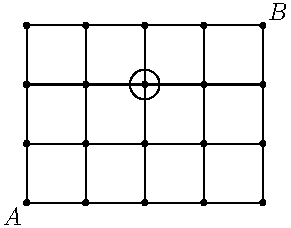
\includegraphics{yip-1-2}
  \]
\end{problem}
\begin{solution*}
  This problem is only slightly more complicated than its predecessor. We
  say slightly because thinking of the circled point as another point \(C\)
  and thinking of paths from \(A\) to \(B\) passing to \(C\) as joining
  paths from \(A\) to \(C\) and paths from \(C\) to \(D\), we have
  \(\binom{4}{2,2}\) ways to get from \(A\) to \(C\) and \(\binom{3}{2,1}\)
  ways to get from \(C\) to \(B\). Thus, we have
  \[
    \binom{4}{2,2}\binom{3}{2,1}
  \]
  paths from \(A\) to \(B\) passing through \(C\).
\end{solution*}

\begin{problem}[Ross, \S 1, \# 33]
  We have \(\$ 20,\!000\) that must be invested among \(4\) possible
  opportunities. Each investment must be integral in units of \(\$1000\),
  and there are minimal investment that need to be made if one is to invest
  these opportunities. The minimal investments are \(\$2000\), \(\$2000\),
  \(\$3000\), and \(\$4000\). How many different investment strategies are
  available if
  \begin{alphlist}
  \item an investment must be made in each opportunity?
  \item investments must be made in at least \(3\) of the \(4\)
    opportunities?
  \end{alphlist}
\end{problem}
\begin{solution*}
  Let us first cut the complexity of the problem by changing translating
  from dollars (\(\$\)) to units (\(1\) unit is \(\$1000\)). Thus, we have
  \(20\) units and we want to distribute them in integers between the \(4\)
  opportunities which require minimal investments of \(2\), \(2\), \(3\),
  and \(4\) units.
  \\\\
  For part (a),
  \\\\
  For part (b),
\end{solution*}

\subsubsection{Theoretical exercises}
\begin{problem}[Ross, \S 1, \# 5]
  Determine the number of vectors \((x_1,\dotsc,x_n)\) such that each
  \(x_k\) is either \(0\) or \(1\) and
  \[
    \sum_{k=1}^n x_k\geq l.
  \]
\end{problem}
\begin{solution*}
\end{solution*}

\begin{problem}[Ross, \S 1, \# 6]
  How many vectors \(x_1,\dotsc,x_k\) are there for which each \(x_k\) is a
  positive integer such that \(1\leq x_k\leq n\) and \(x_1<x_2<\dotsb<
  x_n\)?
\end{problem}
\begin{solution*}
\end{solution*}

\begin{problem}[Ross, \S 1, \# 8]
  Prove that
  \[
    \binom{n+m}{r}=%
    \binom{n}{0}\binom{m}{r}+\binom{n}{1}\binom{m}{r-1}%
    +\dotsb+\binom{n}{r}\binom{m}{0}.
  \]
\end{problem}
\begin{solution*}
\end{solution*}

\begin{problem}[Ross, \S 1, \# 9]
  Use Theoretical Exercise 8 to prove that
  \[
    \binom{2}{n}=\sum_{k=0}^n\binom{n}{k}^2.
  \]
\end{problem}
\begin{solution*}
\end{solution*}

\begin{problem}[Ross, \S 1, \# 12]
  Consider the following combinatorial identity:
  \[
    \sum_{k=1}^n k\binom{n}{k}=n2^{n-1}.
  \]
  \begin{alphlist}
  \item Present a combinatorial argument for this identity by considering
    the set of \(n\) people and determining, in two ways, the number of
    possible selections of a committee of any size and a chairperson for
    the committee.

    \noindent\emph{Hint:}
    \begin{enumerate}[label=(\roman*)]
    \item How many possible elections are there of a committee of size
      \(k\) and its chairperson?
    \item How many possible selections are there of a chairperson and the
      other committee members?
    \end{enumerate}
  \item Verify the following identity for \(n=1,2,3,4,5\):
    \[
      \sum_{k=1}^n \binom{n}{k}k^2=2^{n-2}n(n+1).
    \]
    For a combinatorial proof of the preceding, consider the set of \(n\)
    people and argue that both sides of the identity represent the number
    of different selections of a committee, its chairperson, and its
    secretary (possibly the same as the chairperson).

    \noindent\emph{Hint:}
    \begin{enumerate}[label=(\roman*)]
    \item How many different selection result in the committee containing
      exactly \(k\) people?
    \item How many different selections are there in which the chairperson
      and the secretary are the same? (Answer: \(n2^{n-1}\).)
    \item How many different selections result in a chairperson and the
      secretary being different?
    \end{enumerate}
  \item Now argue that
    \[
      \sum_{k=1}^n\binom{n}{k}k^3=2^{n-3}n^2(n+3).
    \]
  \end{alphlist}
\end{problem}
\begin{solution*}
\end{solution*}

\begin{problem}[Ross, \S 1, \# 23]
  Determine the number of vectors \((x_1,\dotsc,x_n)\) of \(n\) variables
  such that each \(x_k\) is a nonnegative integer and
  \[
    \sum_{k=1}^n x_k\leq l.
  \]
\end{problem}
\begin{solution*}
\end{solution*}

\subsubsection{Problems}
\begin{problem}[Ross, \S 2, \# 25]
  A pair of dice is rolled until a sum of either \(5\) or \(7\)
  appears. Find the probability that a \(5\) occurs first.

  \noindent\emph{Hint:} Let \(E_n\)
  denote the event that a \(5\) occurs on the \(n\)\textsup{th} roll and no
  \(5\) or \(7\) occurs on the first \(n-1\) rolls. Compute \(P(E_n)\) and
  argue that \(\sum_{n=1}^\infty P(E_n)\) is the desired probability.
\end{problem}
\begin{solution*}
\end{solution*}

\begin{problem}[Ross, \S 2, \# 29]
  An urn contains \(n\) white and \(m\) black balls, where \(n\) and \(m\)
  are positive numbers.
  \begin{alphlist}
  \item If two balls are randomly withdrawn, what is the probability that
    they are the same color?
  \item If a ball is randomly withdrawn and then replaced before the second
    one is drawn, what is the probability that the withdrawn balls are the
    same color?
  \item Show that the probability in part (b) is always larger than the one
    in part (a).
  \end{alphlist}
  \end{problem}
\begin{solution*}
\end{solution*}

\begin{problem}[Ross, \S 2, \# 35]
  Seven balls are randomly withdrawn from an urn that contains \(12\) red,
  \(16\) blue, and \(18\) green balls. Find the probability that
  \begin{alphlist}
  \item \(3\) red, \(2\) blue, and \(2\) green balls are withdrawn;
  \item at least \(2\) red balls are withdrawn;
  \item all withdrawn balls are the same color;
  \item either exactly \(3\) red balls or exactly \(3\) blue balls are
    withdrawn.
  \end{alphlist}
\end{problem}
\begin{solution*}
\end{solution*}

\begin{problem}[Ross, \S 2, \# 44]
  Five people, designated as \(A,B,C,D,E\), are arranged in linear
  order. Assuming that each possible order is equally likely, what is the
  probability that
  \begin{alphlist}
  \item there is exactly one person between \(A\) and \(B\)?
  \item there are exactly two people between \(A\) and \(B\)?
  \item there are three people between \(A\) and \(B\)?
  \end{alphlist}
\end{problem}
\begin{solution*}
\end{solution*}

\begin{problem}[Ross, \S 2, \# 49]
  A group of \(6\) men and \(6\) women is randomly divided into \(2\)
  groups of size \(6\) each. What is the probability that both groups will
  have the same number of men?
\end{problem}
\begin{solution*}
\end{solution*}

\subsubsection{Theoretical exercises}
\begin{problem}[Ross, \S 2, \# 5]
  For any sequence of events \(E_1,E_2,\dotsc\), define a new sequence
  \(F_1,F_2,\dotsc\), of disjoint events (that is, events such that
  \(F_j\cap F_k=\emptyset\) whenever \(j\neq k\)) such that for all \(n\geq
  1\),
  \[
    \bigcup_{k=1}^n F_k=\bigcup_{k=1}^n E_k.
  \]
\end{problem}
\begin{solution*}
\end{solution*}

\begin{problem}[Ross, \S 2, \# 14]
  Prove Proposition 4.4 by mathematical induction.
\end{problem}
\begin{solution*}
  Proposition 4.4 is called the inclusion-exclusion identity (or
  inclusion-exclusion principle which the author prefers to use).
  \begin{proposition*}[Inclusion-exclusion identity]
    \[
      \begin{split}
        P(E_1\cup E_2\cup\dotsb\cup E_n)
        =\sum_{k=1}^n P(E_k)&-\sum_{k_1<k_2} P(E_{k_1}\cap E_{k_2})\\
        &+\dotsb+(-1)^{r+1}\sum_{k_1<k_2<\dotsb<k_r}
        P(E_{k_1}\cap\dotsb\cap E_{k_r})\\
        &+\dotsb+(-1)^{n+1}P(E_1\cap\dotsb\cap E_n).
      \end{split}
    \]
    The summation
    \(\sum_{k_1<k_2<\dotsb<k_r}P(E_{k_1}\cap\dotsb\cap E_{k_r})\) is taken
    over all the \(\binom{n}{r}\) possible subsets of size \(r\) of the set
    \(\{1,\dotsc,n\}\).
  \end{proposition*}
\end{solution*}

\begin{problem}[Ross, \S 2, \# 19]
  An urn contains \(n\) red and \(m\) blue balls. They are withdrawn one at
  a time until a total of \(r\), \(r\leq n\), red balls have been
  withdrawn. Find the probability that a total of \(k\) balls are
  withdrawn.

  \noindent\emph{Hint:} A total of \(k\) balls will be withdrawn if there are \(r-1\)
  red balls in the first \(k-1\) withdrawals and the \(k\)\textsup{th}
  withdrawal is a red ball.
\end{problem}
\begin{solution*}
\end{solution*}

%%% Local Variables:
%%% mode: latex
%%% TeX-master: "../MA519-HW-ALL"
%%% End:
